\documentclass[11pt,a4paper]{article}
\usepackage{amsmath,amssymb}
\usepackage{epsfig,graphicx,units,hyperref,subcaption}

\topmargin -0.4cm
\headsep=0.0cm
\headheight=0.0cm
\textheight 24.6cm
\oddsidemargin -0.3cm
\evensidemargin -0.3cm
\textwidth 15.9cm

\begin{document}

\title{\bf Time Stretching of the GeV Emission of GRBs: Fermi LAT data vs geometrical model}
\author{M.~S.~Piskunov$^a$\footnote{{\bf e-mail}: maxitg@icloud.com},
G.~I.~Rubtsov$^{a}$\footnote{{\bf e-mail}: grisha@ms2.inr.ac.ru}
\\
$^a$ \small{\em Institute for Nuclear Research RAS} \\
\small{\em Prospekt 60-letiya Oktyabrya 7a, Moscow 117312}
}
\date{}
\maketitle

\begin{abstract}
Numerous observations confirm that the high energy $(> \unit[100]{MeV})$ emission of gamma ray bursts is delayed with respect to the low energy emission.
However, the difference of light curves in various high energy bands has not been studied properly.

In this paper we consider all the bursts observed by Fermi-LAT since 2008 August 4 to 2011 August 1, for which at least $10$ events with energies $\unit[1]{GeV}$ or higher were observed.
There are $4$ of them: GRB 080916C, GRB 090510, GRB 090902B, and GRB 090926A.
We study their light curves in two bands, $(\unit[100]{MeV}, \unit[1]{GeV})$ and $(\unit[1]{GeV}, \unit[300]{GeV})$.

The Kolmogorov-Smirnov test is used to check whether the light curves for these two bands are the same.
No significant difference was found for GRB 080916C and GRB 090510.
However, we observed with statistical significance of $3.3 \sigma$, that the higher energy light curve of GRB 090926A is stretched with respect to the lower-energy one, and with statistical significance of $2.3 \sigma$, that the lower energy light curve of GRB 090902B is stretched with respect to the higher-energy one.

We suggest a simple geometrical model to explain this result.
The main assumption is the jet opening angle dependence on radiation energy -- the most energetic photons are emitted near the axis of the jet.
We also assume that all bursts are the same in their rest frames (that is their light curves differ only because of different redshifts and different view directions).
To test this model, we compute the total energy of the burst, and confirm that it is below the constraint.
We also compute the fraction of observable bursts in $(\unit[100]{MeV}, \unit[1]{GeV})$ band, which can also be observed in higher energies.
This fraction matches the observations.
We predict the distribution of observable stretching factors, which may be tested in the future when more observational data become available.
Finally, we propose a way to estimate observer's off-axis angles (view directions) based on stretching factors and fractions of high energy photons.

All our code is open source, and is available freely on GitHub\footnote{\url{https://github.com/maxitg/GammaRays}}.
\end{abstract}

\section{Introduction}
Gamma Ray Bursts (GRBs) are among the most energetic events in the Universe, therefore they might provide new knowledge for particle physics.
Modern observatories, specifically Fermi \cite{Ackermann:2012kna} and Swift, \cite{Gehrels:2004gu} made it possible to study these explosions extensively \cite{Vianello:2013ela,Gehrels:2013xd}.
These and previous studies led to several interesting results.
For example, the total energy emitted in gamma-rays during a burst was found to be similar among different bursts within an order of magnitude \cite{Bloom:2003wy}.
This suggests that the majority of the bursts must have similar energetics in their rest frame.
Temporal variations of spectra were also studied.
The spectral lags were found between different low energy bands \cite{Yi:2005ht}.
The very high energy radiation was discovered to be extended relative to the x-ray emission \cite{Castignani:2014gaa,Lange:2013uh,Vianello:2013ela}.
In this study we continue this research and explore the spectral variations between energy bands $(\unit[100]{MeV}, \unit[1]{GeV})$ and $(\unit[1]{GeV}, \unit[300]{GeV})$ (we call them low and high energy bands throughout the paper).
We use the Kolmogorov-Smirnov test to compute the time stretching of radiation in one of these bands compared to the other.
Results obtained with this approach are discussed in section \ref{sec:data}.
Then we propose a simple geometrical model to explain these results in section \ref{sec:model}.
Finally, our study is summarized in section \ref{sec:summary}.

\section{Fermi LAT Data}
\label{sec:data}

We take the GRB list from the Fermi-LAT catalog \cite{Ackermann:2013zfa}, and use the technique introduced in \cite{Rubtsov:2011qq} to estimate background radiation in both energy bands.\footnote{Detailed description of computations in this and the next section can be found in the extended version of the paper on GitHub.}
Most of the bursts in the catalog, however, do not have enough events with over $\unit[1]{GeV}$ energies to do desired computations, so we choose only those bursts, from which at least $10$ photons were detected in the high energy band.
This leaves $4$ of them: 080916C \cite{Tajima:2009az}, 090510 \cite{Ackermann:2010us}, 090902B \cite{Abdo:2009pg} and 090926A \cite{Bregeon:2011bu}.

For these 4 bursts we compute both high and low energy distributions of photon times.
We subtract the low energy background estimate from the low energy CDF, and add the high energy background estimate to it.
This makes the low energy CDF non-monotonous and, rigorously speaking, we cannot use the 2-sample Kolmogorov-Smirnov test on it.
However, since there is a much greater number of photons on lower energies, we can think of the low energy CDF as continuous.
Therefore, this non-monotonicity will be negligible, and will not harm the KS-test results much.

Finally, we stretch the high energy CDF by different factors, and compare it to the low energy CDF using the KS-test.
If we require $2\sigma$-significant probability to exclude a particular stretching factor, then the stretching factor of $1$ (which means no stretching) is allowed for GRBs 080916C and 090510.
For the other two bursts the stretching factor of $1$ is, however, prohibited.
For GRB 090902B, it is smaller than $1$, so the low energy light curve is stretched with respect to high energy one (see fig. \ref{fig:grb090902B}).
And for GRB 090926A, even more dramatic deviation for the stretching factor of $1$ is observed in the opposite direction.
The high energy light curve of GRB 090926A is stretched with respect to low energy one with a factor of at least $1.99$ (see fig. \ref{fig:grb090926A}).
You can see allowed ranges for stretching factors for all the bursts studied in table \ref{tab:bursts}.

\begin{figure}
        \centering
        \begin{subfigure}{0.49\textwidth}
                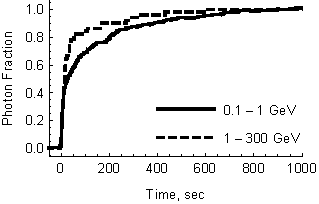
\includegraphics[width=\textwidth]{lightCurve090902B}
                \label{fig:lightCurve090902B}
        \end{subfigure}
        \begin{subfigure}{0.49\textwidth}
                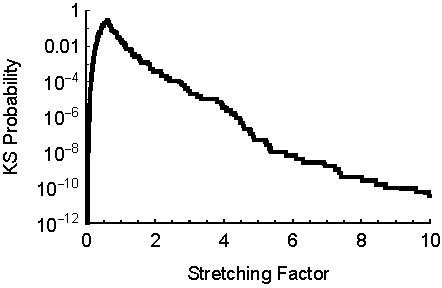
\includegraphics[width=\textwidth]{probabilities090902B}
                \label{fig:probabilities090902B}
        \end{subfigure}
        \caption{GRB 090902B results. Low energy radiation is stretched ($\kappa < 1$) with significance of $2.3\sigma$.}
        \label{fig:grb090902B}
\end{figure}

\begin{figure}
        \centering
        \begin{subfigure}{0.49\textwidth}
                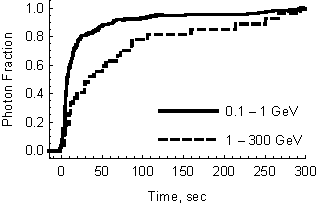
\includegraphics[width=\textwidth]{lightCurve090926A}
                \label{fig:lightCurve090926A}
        \end{subfigure}
        \begin{subfigure}{0.49\textwidth}
                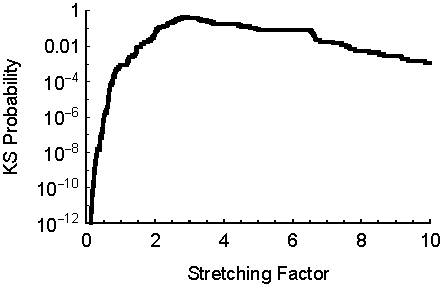
\includegraphics[width=\textwidth]{probabilities090926A}
                \label{fig:probabilities090926A}
        \end{subfigure}
        \caption{GRB 090926A results. High energy radiation is stretched ($\kappa > 1$) with significance of $3.3\sigma$.}
        \label{fig:grb090926A}
\end{figure}

\begin{table}
	\centering
	\small
	\begin{tabular}{ l | c | c | c | c | c | c | c}
		GRB 	& 	Redshift	&	GBM Trigger Time	& R.A., Dec.			&	Stretching factor	&	Stretching factor	\\
		Name 	& 				&	MET sec				& J2000, deg			&	$2\sigma$ range		&	$3\sigma$ range		\\
		\hline
		080916C	&	$4.35$		&	243216766.614		&	119.85,	-56.64 		&	0.67 -- 3.32		&	0.42 -- 5.83		\\
		090510 	&	$0.903$		&	263607781.971		&	333.55, -26.58		&	0.43 -- 1.61		&	0.32 -- 2.29		\\
		090902B	&	$1.822$		&	273582310.313		&	264.94,  27.32		&	0.35 -- 0.89		&	0.22 -- 1.53		\\
		090926A	&	$2.1062$	&	275631628.990		&	353.40, -66.32 		&	1.99 -- 6.62		&	1.34 -- 9.15		\\
	\end{tabular}
	\caption{
		Stretching factor computation results for the bursts studied. Ranges of allowed stretching factors are shown for studied bursts for multiple levels of significance.
		The values for trigger time and location are taken from the tables 2 and 4 of \cite{Ackermann:2013zfa}.
	}
	\label{tab:bursts}
\end{table}

So we obtained a preliminary (note that its significance is less than $5\sigma$) result that the stretching factors for observable bursts might be both larger and smaller than $1$.

\section{Model}
\label{sec:model}

We propose that time stretching of GRB light curves can be explained by the curvature effects (that is the effects of jet geometry) even if all the bursts are the same in their rest frames.
These effects were explored by multiple authors \cite{Nakamura:2001kd,Shen:2005ea,Shenoy:2013cba}.
However, these studies were only concerned with x-ray radiation, and, even more importantly, they assumed that the distribution of radiation sources is homogeneous throughout the jet.
We propose a contrary idea: that the highest energy radiators are concentrated near the axis of the burst, meaning that the burst opening angle depends on energy.
We cannot prove this assumption rigorously, but have arguments supporting it.

First of all, there are around 750 GRBs detected by GBM, half of which were in the LAT field of view at the moment of observation \cite{Vianello:2013ela}.
However, only about 30 of them were detected by the LAT, and only 4 of them were bright in the high energy band.
If we extrapolate the uniform jet model to very high energies, this observation would mean that these groups of bursts are internally different: some of them produce VHE radiation, and other do not.
These differences are hard to explain given that burst energetics are similar \cite{Bloom:2003wy}.
Nevertheless, these differences in burst counts can easily be explained by our model.
In our model, the opening angle of a jet is inversely proportional to the energy of photons it radiates.
Therefore the most common scenario is that the off-axis angle of the observer is smaller than the low energy jet opening angle, but larger than the opening angle of a high energy jet.
Because of that, most of the bursts can only be seen at low energies.
The 4 bursts we study in this paper were seen, according to our model, from the lowest off-axis angles.

Second, consider the plasma right after its ejection from the central engine.
Two processes happen here simultaneously:
\begin{enumerate}
	\item{Particles near the jet boundary change their movement directions, therefore increasing the opening angle of the jet.}
	\item{Particles lose energy, therefore decreasing radiation frequency emitted by the jet.}
\end{enumerate}
We argue that these two processes are correlated, for they happen due to the same particle interaction processes.
And since they are correlated, jets with larger opening angles should have lower energies, which is the assumption we are trying to justify.

You can see why this assumption allows for non-trivial stretching factors in the figure \ref{fig:modelOverview}.
More rigorously, the model is defined by the following assumptions:
\begin{enumerate}
	\item{
		Time $t = 0$, a spherical shell of plasma is emitted.
		The center is called the central engine.
	}
	\item{The shell points propagate with a constant velocity $v = \frac{\sqrt{\gamma^2-1}}{\gamma} \sim 1$, so at the time $t$ the radius of the shall is $v t$.}
	\item{Each point of the shell is an isotropic radiator in its rest frame.}
	\item{
		The radiation intensity is a function of the radiator position and the radiation frequency:
		\begin{equation*}
			\eta\left(r,\theta,\omega\right) = 
			\frac{\eta_0}{1 + \left(\frac{r}{r_0}\right)^n}
			\exp\left(
				-\left(\frac{\theta}{\theta_0}\right)^2
				\left(\frac{\omega}{\omega_0}\right)^{-2k}
			\right)
			\left(\frac{\omega}{\omega_0}\right)^\alpha
		\end{equation*}
		$\eta$ is the number of particles emitted per volume per solid angle per frequency.
		It is a function of the distance $r$ from the central engine, the off-axis angle $\theta$, and the radiation frequency $\omega$.
	}
\end{enumerate}

\begin{figure}
	\centering
	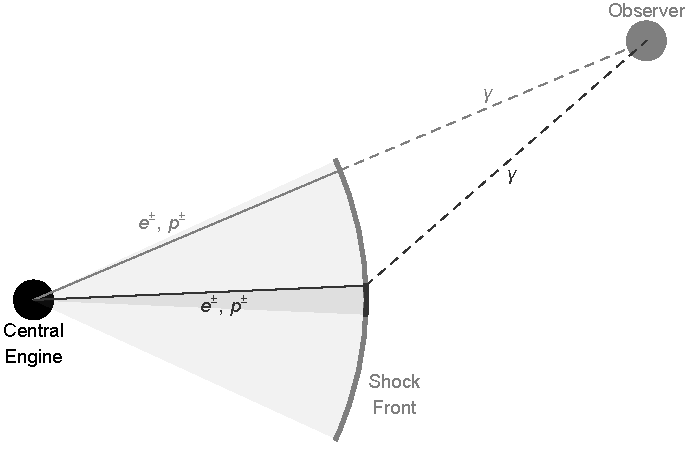
\includegraphics[width=0.7\textwidth]{modelOverview}
	\caption{
        Model Overview.
        Here lighter and darker cones represent the regions through which low and high energy plasma propagates.
        In case depicted the observer's off-axis angle is smaller than the opening angle of the low energy jet, so, due to the relativistic beaming effect, the most of the observable low energy photons will travel along the straight line from the central engine.
        Also, the observer's off-axis angle is larger that the opening angle of the high energy jet, so the high energy radiation will still originate near the center of the jet (because it is the only place where there are high energy radiators).
        The observation time of a photon is a sum of two things: the time interval spent in plasma as a radiator (which approximately equals to the distance from the central engine to the point of emission); and the time interval from emission to detection (which is the distance from the point of emission to the observer's location).
        Given a position of the shock front, this sum is larger for high energy photons.
        Because of that, high energy emission will be observed later throughout the burst duration, therefore the high energy light curve will be stretched.
        }
    \label{fig:modelOverview}
\end{figure}

The burst is fully specified by the following set of parameters (we assume these parameters to be the same for all bursts, the specified values are obtained by fitting to make possible observed bursts from section \ref{sec:data}):
\begin{itemize}
	\item{$\gamma = 300$, the relativistic factor of the shell, $\gamma \gg 1$.}
	\item{$\eta_0 = \unit[4.63 \times 10^{34}]{sec^{-3} GeV^{-1}}$, which defines the luminosity scale.}
	\item{$r_0 = \unit[3.14 \times 10^6]{sec}$, the characteristic jet length; $r_0 \ll \frac{1}{H\left(0\right)}$, $H\left(t\right)$ is the Hubble parameter;}
	\item{$n = 23.0$, which determines the sharpness of the jet end, $n > 3$;}
	\item{$\omega_0 = \unit[1]{GeV}$, a characteristic radiation frequency;}
	\item{$\theta_0 = 7.93 \times 10^{-5}$, the opening angle of the jet for radiation with frequency $\omega_0$, $\theta_0 \ll 1$;}
	\item{$k = -0.654$, which determines how much the opening angle changes with frequency, $k < 0$;}
	\item{$\alpha = -0.724$, the bare spectral index, $\alpha < -2k - 1$}
\end{itemize}

Numerical simulations based on these assumptions are able to reproduce both stretching factors smaller than $1$ (like of GRB 090902B) and larger than $1$ (like of GRB 090926A) depending on redshift and observer's off-axis angle (see fig. \ref{fig:sampleLightCurves}).

\begin{figure}
	\centering
	\hspace*{\fill}
	\begin{subfigure}{0.45\textwidth}
		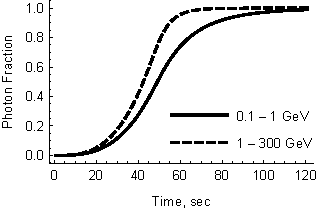
\includegraphics[width=\textwidth]{sampleLightCurveLogNegative}
		\label{fig:sampleLightCurveLogNegative}
		\caption{Stretching factor $\kappa = 0.819$, redshift $z = 1.82$, off-axis angle $\chi = 0$.}
	\end{subfigure}
	\hfill
	\begin{subfigure}{0.45\textwidth}
		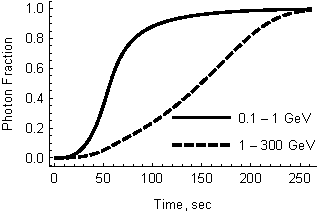
\includegraphics[width=\textwidth]{sampleLightCurveLogPositive}
		\label{fig:sampleLightCurveLogPosivie}
		\caption{Stretching factor $\kappa = 2.43$, redshift $z = 2.106$, off-axis angle $\chi = 5.90 \times 10^{-3}$.}
	\end{subfigure}
	\hspace*{\fill}
	\caption{
		High and low energy light curves produced by the geometrical model.
		Burst parameter values are listed in section \ref{sec:model}.
	}
	\label{fig:sampleLightCurves}
\end{figure}

To test the model against observations, we computed a few more things:
\begin{itemize}
	\item{
		Total energy emitted in $\unit[100]{MeV}$ and more energetic gamma rays $E < \unit[5.89 \times 10^{53}]{GeV}$, which is in agreement with \cite{Gehrels:2013xd}.
	}
	\item{
		Distribution of stretching factors of observable bursts.
		You can see the PDF and the CDF of it on fig. \ref{fig:kappaDistribution}.
		This distribution doesn't contradict with the values of stretching factors obtained in section \ref{sec:data}.
	}
	\item{
		The fraction of bursts observable in low energy band, which are also observed in high energy band $f_m = 0.110$.
		The Fermi LAT catalog contains $35$ bursts out of which $4$ can be observed in high energy band.
		Therefore the observed value $f_o = 0.11 \pm 0.05$ (error obtained from binomial distribution) agrees with the model.
	}
	\item{
		There is a correlation between the fraction of high energy photons (that is high energy photon count divided by the total photon count), the stretching factor and the observer's off-axis angle (see fig. \ref{fig:correlations}). It allows one to predict observer's off-axis angles.
	}
\end{itemize}

\begin{figure}
	\hspace*{\fill}
	\begin{subfigure}{0.45\textwidth}
		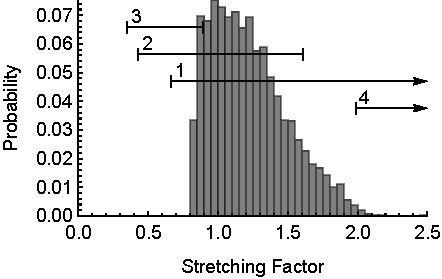
\includegraphics[width=\textwidth]{kappaDistributionHistogram}
		\label{fig:kappaDistributionHistogram}
		\caption{Histogram obtained from the model. Error bars show observed stretching factors.}
	\end{subfigure}
	\hfill
	\begin{subfigure}{0.45\textwidth}
		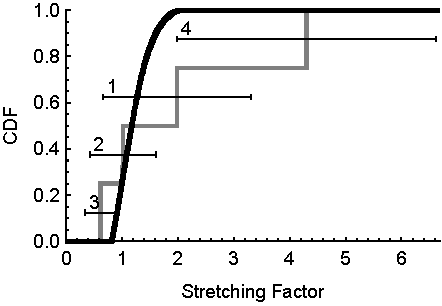
\includegraphics[width=\textwidth]{kappaDistributionCDF}
		\label{fig:kappaDistributionCDF}
		\caption{CDF obtained from the model. Steps and error bars show observed stretching factors.}
	\end{subfigure}
	\hspace*{\fill}
	\caption{
		Stretching factors histogram and CDF produced by our model.
		The sample contains $4096$ bursts.
		Numbered error bars correspond respectively to GRB 080916C, GRB 090510, GRB 090902B and GRB 090926A.
	}
	\label{fig:kappaDistribution}
\end{figure}

\begin{figure}
        \centering
        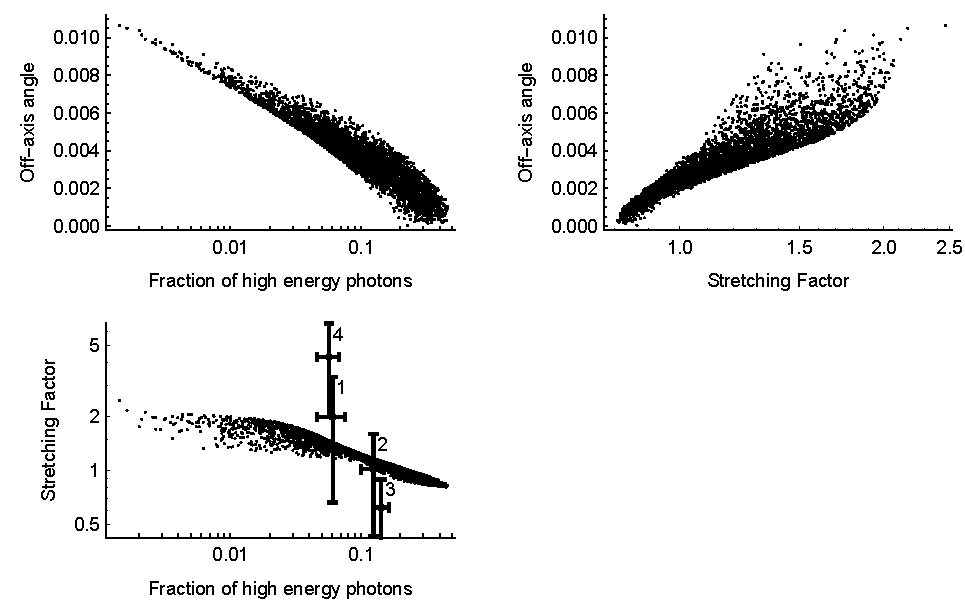
\includegraphics[width=1.0\textwidth]{correlations}
        \caption{
        	Correlations between off-axis angles, stretching factors and high to low energy photon count ratios found in the sample produced by our model.
        	The sample contains $4096$ bursts.
        	Numbered black crosses show data respectively for GRB 080916C, GRB 090510, GRB 090902B and GRB 090926A with $2\sigma$ error bars.
        	This correlation allows one to estimate off-axis angles of observed bursts.
        }
        \label{fig:correlations}
\end{figure}

So our model, though with some discrepancies, is able to explain the time stretching result from section \ref{sec:data}.

\section{Summary}

\label{sec:summary}
	
Our study can be summarized in 3 main points.

First, the time stretching of GRB light curves between different VHE bands, in particular $(\unit[100]{MeV}, \unit[1]{GeV})$ and $(\unit[1]{GeV}, \unit[300]{GeV})$, is discovered with statistical significance of $3.3\sigma$.
This time stretching might be positive or negative (that is higher or lower energy light curve is stretched) depending on the burst.

Second, this time stretching effect can be explained with curvature effects, that is effects of jet geometry.
There is no need to introduce any new spectral components.

Finally, we can assume all GRBs to be the same in their rest frames.
The internal burst parameters (such as $\gamma$, $\eta_0$, $r_0$, $n$, $\omega_0$, $\theta_0$, $k$ and $\alpha$) might stay the same for all bursts, and this assumption is more or less consistent with existing observations.

However, there are some caveats, and directions for improvement.

First of all, the model prediction and observations are not completely consistent.
If you look at fig. \ref{fig:correlations}, you will see that the stretching factor of GRB 090926A is too high compared to the model prediction.
It appears that parameters of the model cannot be fitted to account for it (without ruining agreement with other observations).
More data should be analyzed to see whether the problem will be exacerbated, and some refinement of the model might also be required.

Second, the shapes of light curves produced by the model (see fig. \ref{fig:sampleLightCurves}) differ considerably from observed ones (e.g. fig. \ref{fig:grb090902B}).
Most importantly, the slope of light curves produced by the model is zero at $t = 0$, even though the slope of observed light curves at $t = 0$ is not only non-zero, but appears to have a maximum.

Third, the assumption of plasma energy dependence on off-axis angle should be better justified.
This might probably be done using hydrodynamic simulation of the jet.

Finally, even though it appears that bursts are similar in their rest frames, they cannot be exactly the same.
The differences in masses, metallicities, angular momenta of progenitor stars, and the differences in local conditions around them might account for differences in light curves of GRBs (or, even, for especially large stretching factor of GRB 090926A).
It means that minor variations of model parameters might be necessary on burst per burst basis.

It seems, however, that all these problems are not unresolvable, and may be addressed by refining the model without changing its main assumptions.

{\small {\it Acknowledgments.} The work was supported by Russian Science Foundation grant 14-12-01340.}

\bibliographystyle{plain}
\bibliography{piskunov}

\end{document}